\chapter{Resultados y análisis}

\section{Verificación del sistema}

La ejecución de \texttt{make check} finalizó correctamente sobre la versión
integrada desde \texttt{main}. Se compilaron el monitor y los tres simuladores.
\texttt{tests/test\_motor\_deteccion} validó persistencia, escalamiento a
crítica y correlación de archivos; \texttt{tests/test\_respuesta} comprobó que
el modo \texttt{alerta} no envía señales y que \texttt{terminar\_lab} rechaza
alertas no críticas, PID~1, PGID inválidos, PGID no autorizado, UID incorrecto e
identidad obsoleta (\texttt{starttime}). También se validó la sintaxis de los
scripts y la política estática de contención en \texttt{respuesta.c}. Esta
verificación confirma el funcionamiento esperado del código refactorizado, pero
no sustituye las mediciones experimentales en las VM.

Las capturas registraron líneas base de 106 y 104 procesos, con 24,28\% y
23,86\% de RAM, respectivamente. No se dispone de una corrida independiente de
actividad normal con el monitor activo; por ello, no se calcula una tasa de
falsos positivos ni la sobrecarga del monitor.

\section{Funcionamiento ante proliferación de procesos}

\subsection{Prueba 1: carga moderada}

La primera corrida permitió observar la degradación inicial de la máquina
virtual durante la proliferación de procesos. La configuración y el estado
previo a la ejecución se muestran en la Figura~\ref{fig:fork-p1-inicio}. El
recolector tomó 55 muestras, con una línea base de 106 procesos y un máximo de
236. Durante la prueba, el uso máximo de CPU alcanzó 57,14\% y la RAM aumentó
de 24,28\% a 37,77\%, como resume la
Figura~\ref{fig:fork-p1-resultados}. Esta corrida muestra una carga moderada:
el número de procesos y el consumo de recursos aumentaron, pero no alcanzaron
la severidad observada en la segunda prueba.

\begin{figure}[H]
  \centering
  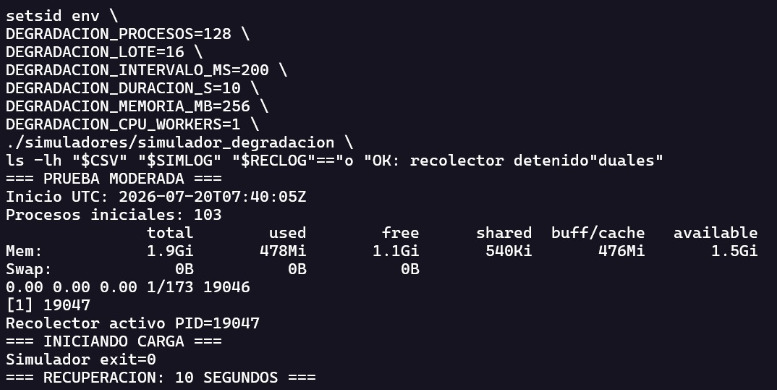
\includegraphics[width=0.94\textwidth]{figuras/anexos/fork_prueba_1_inicio.png}
  \caption{Prueba 1: configuración, línea base e inicio de la carga moderada.}
  \label{fig:fork-p1-inicio}
\end{figure}

\begin{figure}[H]
  \centering
  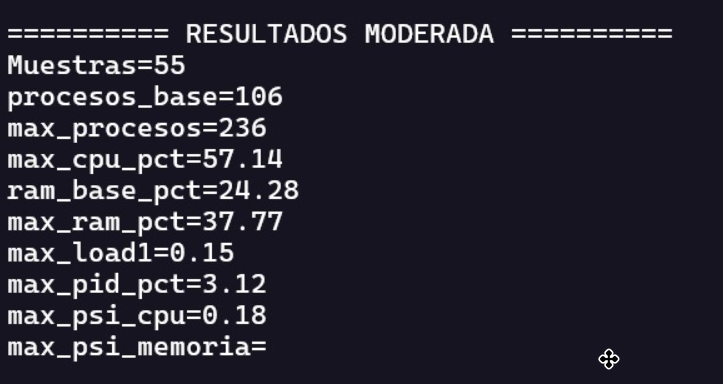
\includegraphics[width=0.94\textwidth]{figuras/anexos/fork_prueba_1_resultados.png}
  \caption{Prueba 1: resumen de mediciones de la carga moderada.}
  \label{fig:fork-p1-resultados}
\end{figure}

\subsection{Prueba 2: carga crítica}

La segunda corrida con fork bomb quedó incorporada al informe como evidencia
de carga crítica. La captura inicial registró 101 procesos
(Figura~\ref{fig:fork-p2-inicio}); el resumen del recolector reportó una línea
base de 104, un máximo de 619 procesos, CPU máxima de 100\% y uso máximo de RAM
de 73\% (Figura~\ref{fig:fork-p2-resultados}). Una captura adicional mostró 616
procesos y 1,4 GiB de memoria usada sobre 1,9 GiB disponibles en la máquina
virtual (Figura~\ref{fig:fork-p2-estado}). Estas observaciones corresponden a
una corrida y se conservarán como evidencia preliminar hasta completar las
repeticiones del protocolo.

\subsection{Evidencia con Anti-Bunny Virus activo}

La Figura~\ref{fig:sistema-anti-activo} muestra la salida del monitor durante
la carga de procesos. El archivo JSON asociado contiene 14 alertas de tipo
\texttt{procesos}, correspondientes a siete PID distintos del usuario
\texttt{antibunny-test}. Todos pertenecen al PGID 12480 y se ejecutaron en modo
\texttt{alerta}; por tanto, esta corrida permite evaluar la detección, pero no
la contención mediante señales.

\begin{figure}[H]
  \centering
  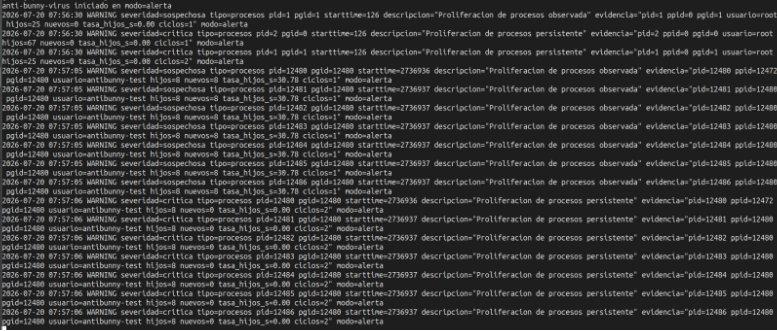
\includegraphics[width=\textwidth]{figuras/resultados/sistema_anti.png}
  \caption{Registro de Anti-Bunny Virus durante la detección de proliferación de procesos.}
  \label{fig:sistema-anti-activo}
\end{figure}

\begin{table}[H]
  \centering
  \caption{Resumen de eventos obtenidos del log JSON del sistema protegido.}
  \label{tab:eventos-antibunny}
  \small
  \begin{tabular}{p{0.43\textwidth}p{0.42\textwidth}}
    \toprule
    Indicador & Valor observado \\
    \midrule
    Intervalo registrado & 20-07-2026, 07:57:05--07:57:06 \\
    Eventos totales & 14 alertas \texttt{WARNING} \\
    Procesos distintos & 7 PID \\
    Grupo y usuario & PGID 12480; \texttt{antibunny-test} \\
    Primer ciclo & 7 alertas sospechosas; 8 hijos nuevos por PID \\
    Tasa máxima observada & 30,78 hijos/s \\
    Segundo ciclo & 7 alertas críticas por persistencia \\
    Modo de respuesta & \texttt{alerta}; sin terminación registrada \\
    \bottomrule
  \end{tabular}
\end{table}

La Figura~\ref{fig:evolucion-hijos-json} muestra la evolución por proceso que
puede reconstruirse del JSON. En el primer ciclo, cada uno de los siete PID
tenía ocho hijos y había creado ocho hijos nuevos, con una tasa máxima de 30,78
hijos/s; el sistema emitió una alerta sospechosa. En el segundo ciclo se
mantuvieron los ocho hijos, no aparecieron hijos nuevos y la persistencia elevó
la alerta a crítica. La caída de hijos nuevos a cero no demuestra que
Anti-Bunny Virus detuviera la carga: el log conserva ocho hijos por PID y fue
generado en modo \texttt{alerta}, sin señales de terminación.

\begin{figure}[H]
  \centering
  \begin{tikzpicture}
    \begin{axis}[
      ybar=2pt,
      width=0.88\textwidth,
      height=0.43\textwidth,
      bar width=24pt,
      ymin=0,
      ymax=9,
      ytick={0,1,...,9},
      xtick={1,2},
      xticklabels={Ciclo 1: sospechosa,Ciclo 2: crítica},
      xlabel={Ciclo de persistencia},
      ylabel={Hijos por proceso alertado},
      legend style={at={(0.5,1.02)},anchor=south,legend columns=2},
      grid=major,
      nodes near coords,
      enlarge x limits=0.35
    ]
      \addplot table[x=ciclo,y=hijos_por_pid,col sep=comma]
        {datos/anti_bunny_hijos_por_ciclo.csv};
      \addplot table[x=ciclo,y=nuevos_por_pid,col sep=comma]
        {datos/anti_bunny_hijos_por_ciclo.csv};
      \legend{Hijos presentes,Hijos nuevos}
    \end{axis}
  \end{tikzpicture}
  \caption{Evolución de hijos por proceso y escalamiento de la detección según el log JSON.}
  \label{fig:evolucion-hijos-json}
\end{figure}

\section{Comparación e interpretación}

La Tabla~\ref{tab:comparacion-resultados} resume las dos corridas sin protección
y la corrida con detección activa. El JSON protegido no registra procesos
totales, CPU ni RAM global.

\begin{table}[H]
  \centering
  \caption{Resumen de las corridas documentadas.}
  \label{tab:comparacion-resultados}
  \small
  \begin{tabular}{p{0.25\textwidth}p{0.20\textwidth}p{0.20\textwidth}p{0.22\textwidth}}
    \toprule
    Indicador & Prueba 1 & Prueba 2 & Anti-Bunny activo \\
    \midrule
    Condición & Sin monitor & Sin monitor & Modo \texttt{alerta} \\
    Procesos base & 106 & 104 & No registrado \\
    Máximo de procesos & 236 & 619 & No registrado \\
    Incremento respecto a base & 122,64\% & 495,19\% & No calculable \\
    CPU máxima & 57,14\% & 100\% & No registrada \\
    RAM inicial--máxima & 24,28--37,77\% & 23,86--73\% & No registrada \\
    Evidencia de detección & No aplica & No aplica & 7 sospechosas y 7 críticas \\
    Evidencia de contención & No aplica & No aplica & No; modo \texttt{alerta} \\
    \bottomrule
  \end{tabular}
\end{table}

\begin{itemize}
  \item Prueba 1: aumento de 130 procesos y 13,49 puntos porcentuales de RAM.
  \item Prueba 2: aumento de 515 procesos, CPU máxima de 100\% y aumento de
        49,14 puntos porcentuales de RAM.
  \item Anti-Bunny activo: siete PID pasaron de sospechosos a críticos en dos
        ciclos, con una tasa máxima de 30,78 hijos/s. No hubo contención porque
        el sistema operó en modo \texttt{alerta}.
\end{itemize}

\section{Hipótesis y limitaciones}

\textbf{Resultado de la hipótesis:} respaldo parcial. Se verificaron la
detección de procesos, el escalamiento por persistencia y los rechazos de
seguridad automatizados.

\textbf{Limitaciones:}
\begin{itemize}
  \item Dos corridas sin protección y una con detección; sin tres repeticiones
        equivalentes.
  \item Sin mediciones experimentales de memoria, archivos, falsos positivos,
        sobrecarga, contención o recuperación.
  \item Resultados limitados al entorno de VM y sin validación frente a malware
        real.
\end{itemize}
